% {\sloppy
% \section{Validación experimental}\label{sec:experimentos}

% \subsection{Metodología}

% \paragraph{Implementación.} Los algoritmos están en \texttt{code/algoritmos.py} y siguen línea a línea los Algoritmos~\ref{alg:reparto}, \ref{alg:exacto} y~\ref{alg:voraz}. Los experimentos están en \texttt{code/experimentos.py}, que genera las tablas (\texttt{code/resultados.json}) y las gráficas (\texttt{img/}). Se ejecutaron con Python 3.13 en un procesador Intel Xeon de 2.8\,GHz.

% \paragraph{Instancias sintéticas (reproducibles).} Todas las instancias se generan con semillas fijas (semilla base $2026$):
% \begin{itemize}
%   \item \textbf{Parte 1.} Pesos $w_i\sim U[1,100]$ y utilidad $u_i(x)=w_i\ln(1+x)$, creciente y cóncava, evaluable en $O(1)$.
%   \item \textbf{Parte 2.} Utilidad de cobertura. Cada nodo $j$ tiene un conjunto $S_j$ de categorías elegidas al azar de un universo $U$, con $|S_j|$ aleatorio entre $s_{\min}$ y $s_{\max}$.
% \end{itemize}

% \paragraph{Medición.} Cada punto es la \textbf{mediana} de 5 ejecuciones (3 para el exacto) medidas con \texttt{time.perf\_counter}, con el recolector de basura desactivado durante la medición, como hace \texttt{timeit}. Se usan entre 6 y 7 tamaños por experimento, duplicando el tamaño en cada paso.

% \paragraph{Contraste con la teoría.} Para cada tamaño se calcula el cociente
% \[
% r = \frac{T_{\text{medido}}}{g},
% \]
% donde $g$ es la función de la cota $\Theta$ deducida. Si la deducción es correcta, $r$ se mantiene aproximadamente constante al crecer el tamaño. En las gráficas, los puntos son los tiempos medidos y la línea es $c\cdot g$, con $c$ igual a la media geométrica de los cocientes $r$ (ajuste por mínimos cuadrados en escala logarítmica). En escala log--log, un costo $n^a$ se ve como una recta de pendiente $a$.

% \subsection{Crecimiento teórico}

% La Figura~\ref{fig:teorico} compara el número de evaluaciones de $f$ que predicen las cotas de la Sección~\ref{sec:exacto} y la Sección~\ref{sec:voraz} con $k=N/2$.

% \begin{figure}[H]
% \centering
% \begin{tikzpicture}
% \begin{semilogyaxis}[
%   width=0.8\linewidth, height=6cm,
%   xlabel={$N$}, ylabel={evaluaciones de $f$},
%   legend pos=north west, legend style={font=\small},
%   grid=major, domain=2:30, samples=29]
%   \addplot[thick,color=red!70!black] {2^x};
%   \addlegendentry{$2^N$ (exacto, todos los subconjuntos)}
%   \addplot[thick,dashed,color=institucional] {x*(x/2)};
%   \addlegendentry{$N\cdot k$ con $k=N/2$ (voraz)}
% \end{semilogyaxis}
% \end{tikzpicture}
% \caption{Crecimiento teórico (escala logarítmica): exponencial frente a polinomial.}
% \label{fig:teorico}
% \end{figure}

% %% ---------------------------------------------------------------------
% \subsection{Parte 1: reparto voraz}

% \paragraph{Optimalidad.} Antes de medir tiempos se comprobó el Teorema~\ref{teo:optimo} contra fuerza bruta: en \textbf{200 instancias} pequeñas ($2\le N\le 4$, $1\le B\le 8$) que enumeran todos los repartos con $\sum_i x_i\le B$, el voraz obtuvo la utilidad óptima en \textbf{200 de 200}.

% \paragraph{Variando $B$ con $N=1000$ fijo.} La teoría predice crecimiento lineal en $B$.

% \begin{table}[H]
% \centering
% \caption{Parte 1 con $N$ fijo. Teoría: $g(N,B)=N+B\log_2 N$.}
% \begin{tabular}{rrrr}
% \toprule
% \rowcolor{uccielo} $N$ & $B$ & $T_{\text{medido}}$ (ms) & $r=T/g$ \\
% \midrule
% 1\,000 & 10\,000 & 7.7 & $7.66\times10^{-8}$ \\
% 1\,000 & 20\,000 & 14.6 & $7.31\times10^{-8}$ \\
% 1\,000 & 40\,000 & 28.8 & $7.20\times10^{-8}$ \\
% 1\,000 & 80\,000 & 59.1 & $7.41\times10^{-8}$ \\
% 1\,000 & 160\,000 & 116.0 & $7.27\times10^{-8}$ \\
% 1\,000 & 320\,000 & 240.2 & $7.53\times10^{-8}$ \\
% \bottomrule
% \end{tabular}
% \end{table}

% \paragraph{Variando $N$ con $B=10N$.} La teoría predice $\Theta(N + B\log N)=\Theta(N\log N)$.

% \begin{table}[H]
% \centering
% \caption{Parte 1 con $B=10N$. Teoría: $g(N,B)=N+B\log_2 N$.}
% \begin{tabular}{rrrr}
% \toprule
% \rowcolor{uccielo} $N$ & $B$ & $T_{\text{medido}}$ (ms) & $r=T/g$ \\
% \midrule
% 1\,000 & 10\,000 & 7.5 & $7.47\times10^{-8}$ \\
% 2\,000 & 20\,000 & 16.0 & $7.24\times10^{-8}$ \\
% 4\,000 & 40\,000 & 34.2 & $7.09\times10^{-8}$ \\
% 8\,000 & 80\,000 & 75.8 & $7.25\times10^{-8}$ \\
% 16\,000 & 160\,000 & 220.2 & $9.79\times10^{-8}$ \\
% 32\,000 & 320\,000 & 582.1 & $1.21\times10^{-7}$ \\
% 64\,000 & 640\,000 & 1547.9 & $1.51\times10^{-7}$ \\
% \bottomrule
% \end{tabular}
% \end{table}

% \begin{figure}[H]
% \centering
% 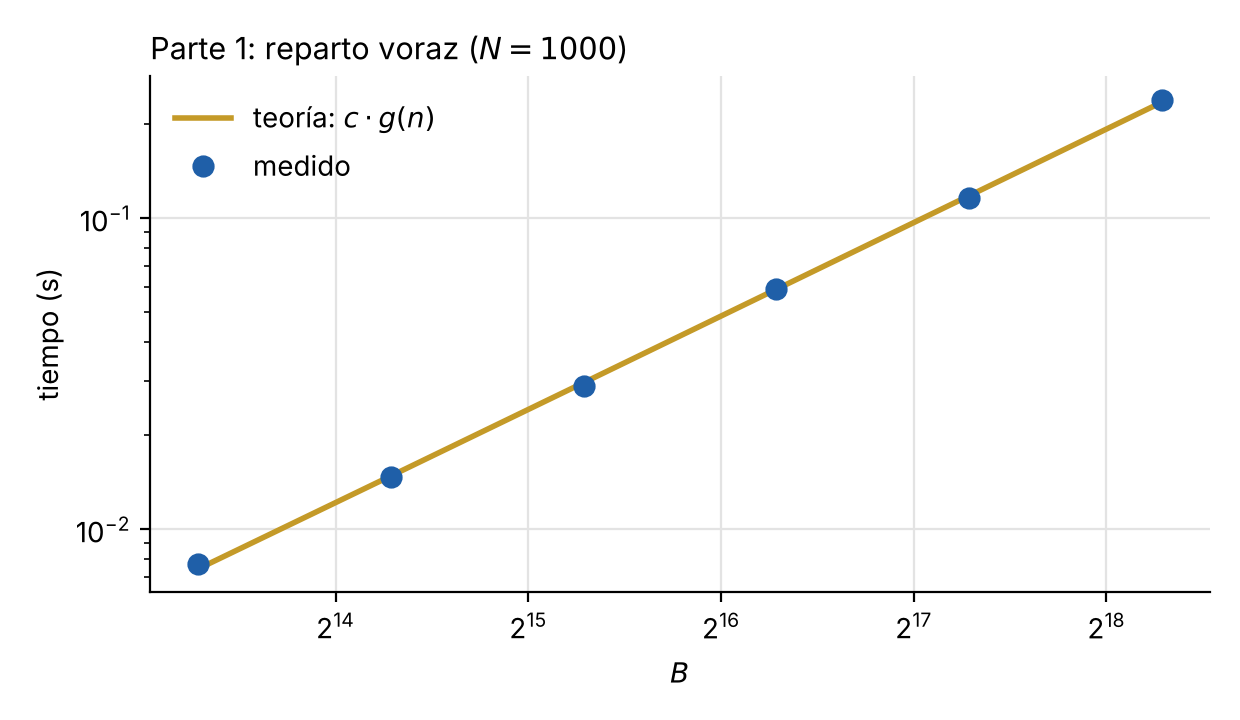
\includegraphics[width=0.49\linewidth]{img/reparto_B.png}\hfill
% 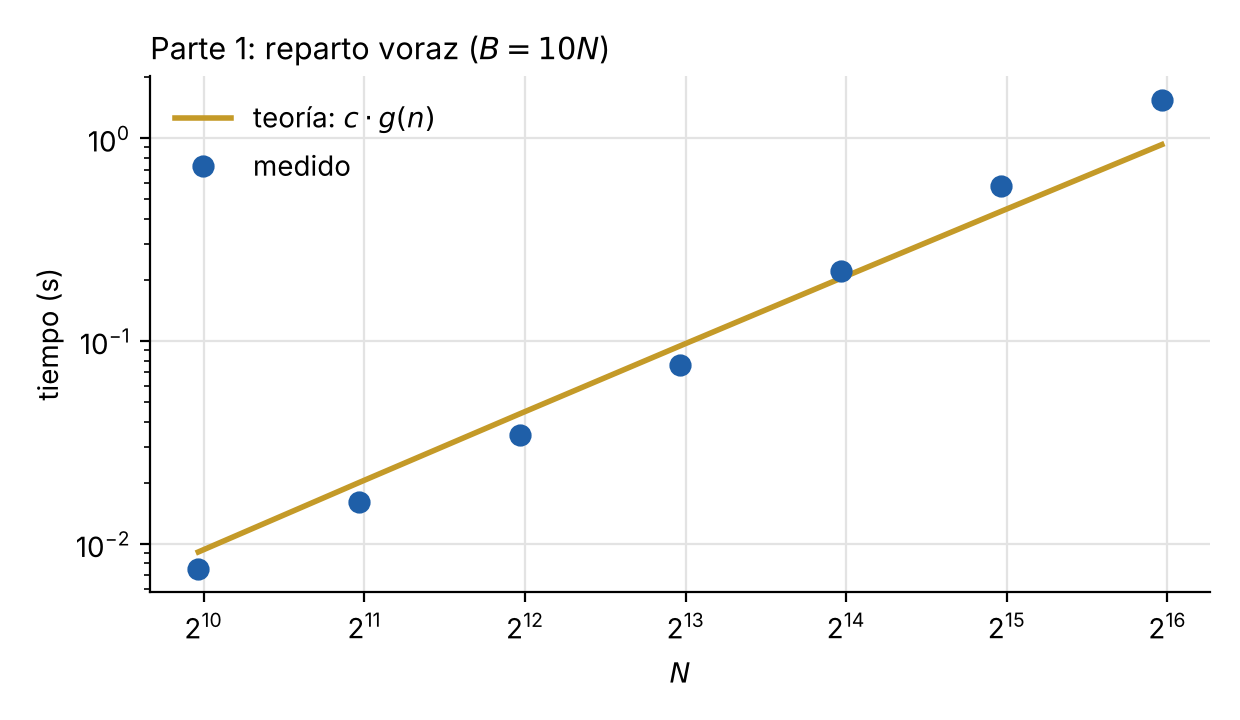
\includegraphics[width=0.49\linewidth]{img/reparto_N.png}
% \caption{Parte 1: tiempo medido (puntos) frente a $c\cdot(N+B\log_2 N)$ (línea), en escala log--log.}
% \label{fig:reparto}
% \end{figure}

% \paragraph{Análisis.} Con $N$ fijo, el cociente $r$ se mantiene en $(7.2$--$7.7)\times10^{-8}$ y la pendiente log--log es 0.99: el tiempo es \textbf{lineal en $B$}, como predice el término $B\log N$. Con $B=10N$, el cociente es estable hasta $N=8000$ y luego crece hasta duplicarse en $N=64\,000$. La causa no es el algoritmo sino la memoria: el análisis supone el modelo RAM, en el que todo acceso cuesta lo mismo, pero cuando el montículo deja de caber en la memoria caché del procesador, cada acceso de \textsc{Extraer-Máximo} e \textsc{Insertar} se vuelve más lento. El crecimiento observado sigue siendo cercano a $N\log N$ (un factor $206$ al multiplicar $N$ por $64$, frente a $102$ predicho, con el factor 2 explicado por la caché) y está muy lejos de un crecimiento cuadrático, que daría un factor $4096$.

% %% ---------------------------------------------------------------------
% \subsection{Parte 2: selección voraz}

% Universo $|U|=1000$ y $|S_j|\in[10,30]$, de modo que $\tau=O(s)$ con $s\le 30$ constante. La columna ``evaluaciones'' cuenta las ganancias $\Delta_j(A)$ calculadas por el programa, y coincide exactamente con la fórmula $kN-k(k-1)/2$ de la Sección~\ref{sec:voraz}.

% \begin{table}[H]
% \centering
% \caption{Selección voraz con $k=20$ fijo. Teoría: $g=kN-k(k-1)/2$.}
% \begin{tabular}{rrrrr}
% \toprule
% \rowcolor{uccielo} $N$ & $k$ & evaluaciones & $T_{\text{medido}}$ (ms) & $r=T/g$ \\
% \midrule
% 500 & 20 & 9\,810 & 11.7 & $1.19\times10^{-6}$ \\
% 1\,000 & 20 & 19\,810 & 24.2 & $1.22\times10^{-6}$ \\
% 2\,000 & 20 & 39\,810 & 53.5 & $1.34\times10^{-6}$ \\
% 4\,000 & 20 & 79\,810 & 104.2 & $1.31\times10^{-6}$ \\
% 8\,000 & 20 & 159\,810 & 209.0 & $1.31\times10^{-6}$ \\
% 16\,000 & 20 & 319\,810 & 416.9 & $1.30\times10^{-6}$ \\
% \bottomrule
% \end{tabular}
% \end{table}

% \begin{table}[H]
% \centering
% \caption{Selección voraz con $N=2000$ fijo. Teoría: $g=kN-k(k-1)/2$.}
% \begin{tabular}{rrrrr}
% \toprule
% \rowcolor{uccielo} $N$ & $k$ & evaluaciones & $T_{\text{medido}}$ (ms) & $r=T/g$ \\
% \midrule
% 2\,000 & 10 & 19\,955 & 27.2 & $1.37\times10^{-6}$ \\
% 2\,000 & 20 & 39\,810 & 51.4 & $1.29\times10^{-6}$ \\
% 2\,000 & 40 & 79\,220 & 84.2 & $1.06\times10^{-6}$ \\
% 2\,000 & 80 & 156\,840 & 141.3 & $9.01\times10^{-7}$ \\
% 2\,000 & 160 & 307\,280 & 248.9 & $8.10\times10^{-7}$ \\
% 2\,000 & 320 & 588\,960 & 462.7 & $7.86\times10^{-7}$ \\
% \bottomrule
% \end{tabular}
% \end{table}

% \begin{figure}[H]
% \centering
% 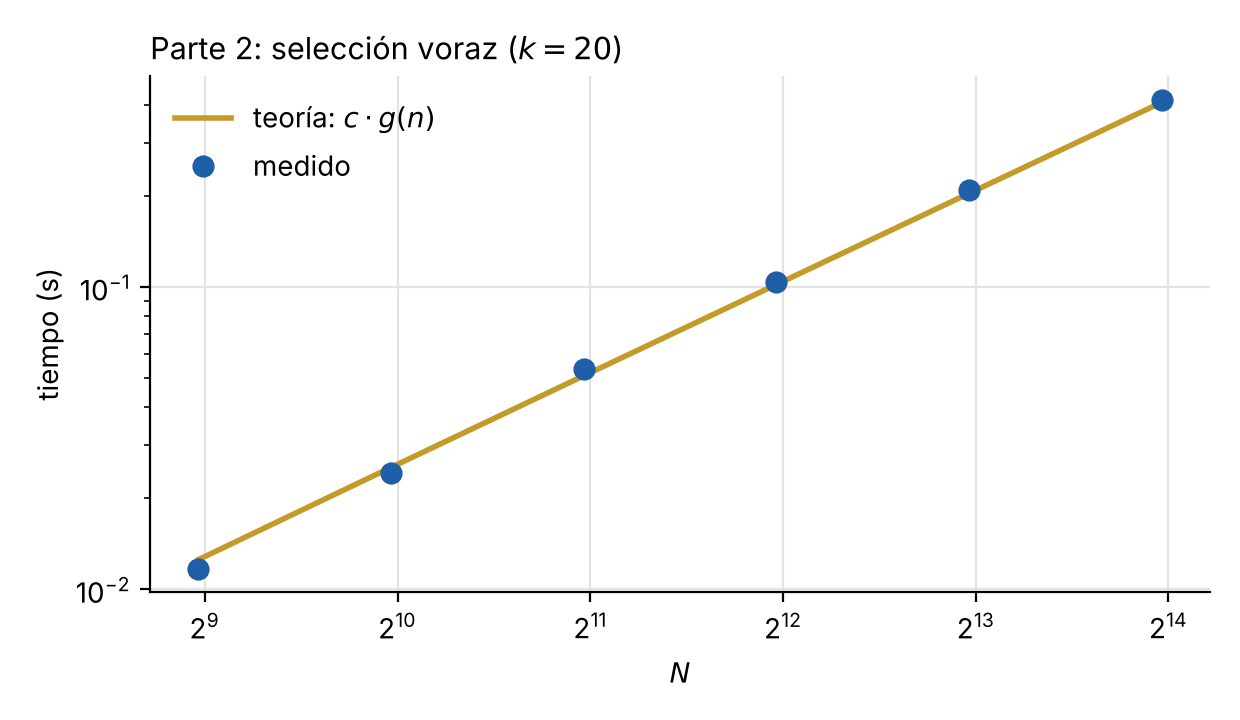
\includegraphics[width=0.49\linewidth]{img/voraz_N.png}\hfill
% 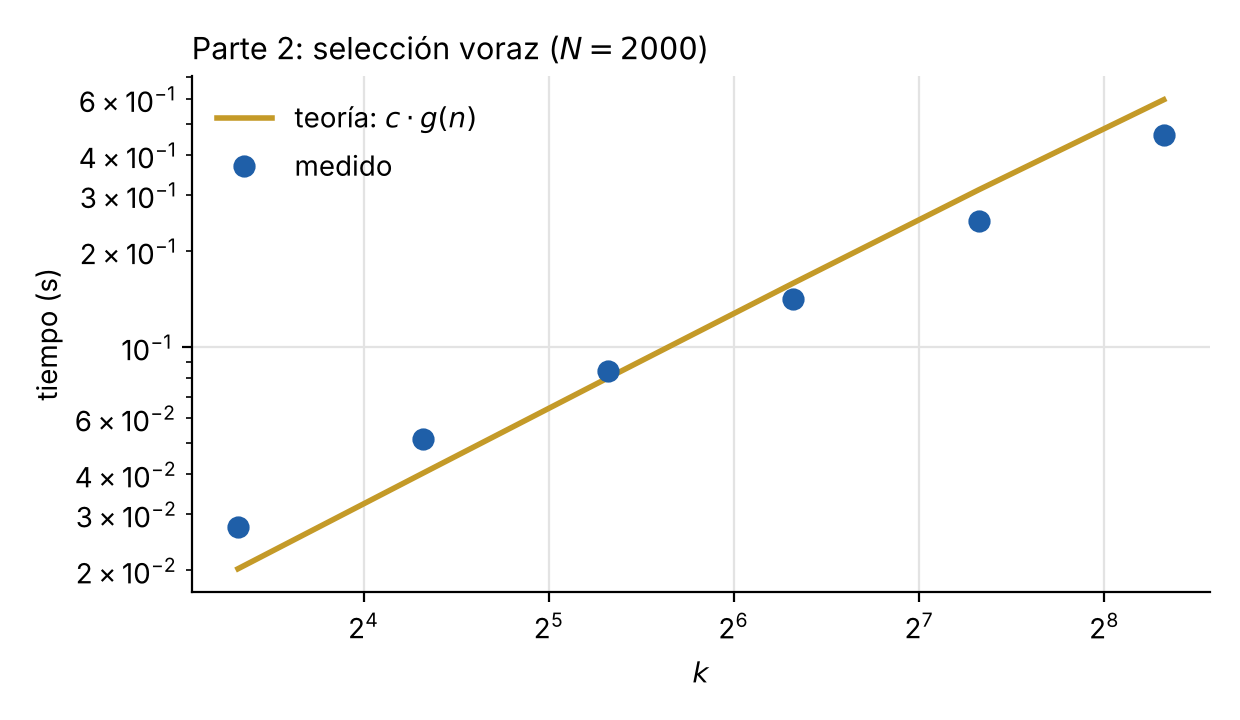
\includegraphics[width=0.49\linewidth]{img/voraz_k.png}
% \caption{Selección voraz: tiempo medido frente a $c\cdot(kN-k(k-1)/2)$, en escala log--log.}
% \label{fig:voraz}
% \end{figure}

% \paragraph{Análisis.} Con $k$ fijo, $r$ es prácticamente constante ($\approx1.3\times10^{-6}$\,s por evaluación) y la pendiente log--log es 1.03: el tiempo es \textbf{lineal en $N$}. Con $N$ fijo, la pendiente es 0.82, algo menor que 1, y $r$ baja de $1.4$ a $0.8\times10^{-6}$. La razón es que $\tau=O(s)$ es una cota superior: cuando $k$ es grande casi todas las categorías ya están cubiertas, y calcular $S_j\setminus C(A)$ produce conjuntos pequeños, que son más baratos de construir. El número de evaluaciones sí sigue exactamente $\Theta(Nk)$.

% %% ---------------------------------------------------------------------
% \subsection{Parte 2: selección exacta}

% Instancias con $|U|=60$, $|S_j|\in[3,8]$ y $k=N/2$, el caso más costoso (Lema~\ref{lem:binom}). Cada hoja calcula $f$ desde cero con $\tau=O(k\,s)$, así que se compara contra $g=\binom{N}{k}\cdot k$.

% \begin{table}[H]
% \centering
% \caption{Selección exacta con $k=N/2$. Teoría: $\binom{N}{k}$ evaluaciones; $g=\binom{N}{k}\,k$.}
% \begin{tabular}{rrrrrr}
% \toprule
% \rowcolor{uccielo} $N$ & $k$ & $\binom{N}{k}$ & evaluaciones & $T_{\text{medido}}$ (ms) & $r=T/g$ \\
% \midrule
% 8 & 4 & 70 & 70 & 0.204 & $7.29\times10^{-7}$ \\
% 10 & 5 & 252 & 252 & 0.458 & $3.63\times10^{-7}$ \\
% 12 & 6 & 924 & 924 & 1.5 & $2.70\times10^{-7}$ \\
% 14 & 7 & 3\,432 & 3\,432 & 5.7 & $2.38\times10^{-7}$ \\
% 16 & 8 & 12\,870 & 12\,870 & 22.6 & $2.20\times10^{-7}$ \\
% 18 & 9 & 48\,620 & 48\,620 & 96.2 & $2.20\times10^{-7}$ \\
% 20 & 10 & 184\,756 & 184\,756 & 371.8 & $2.01\times10^{-7}$ \\
% \bottomrule
% \end{tabular}
% \end{table}

% \begin{figure}[H]
% \centering
% 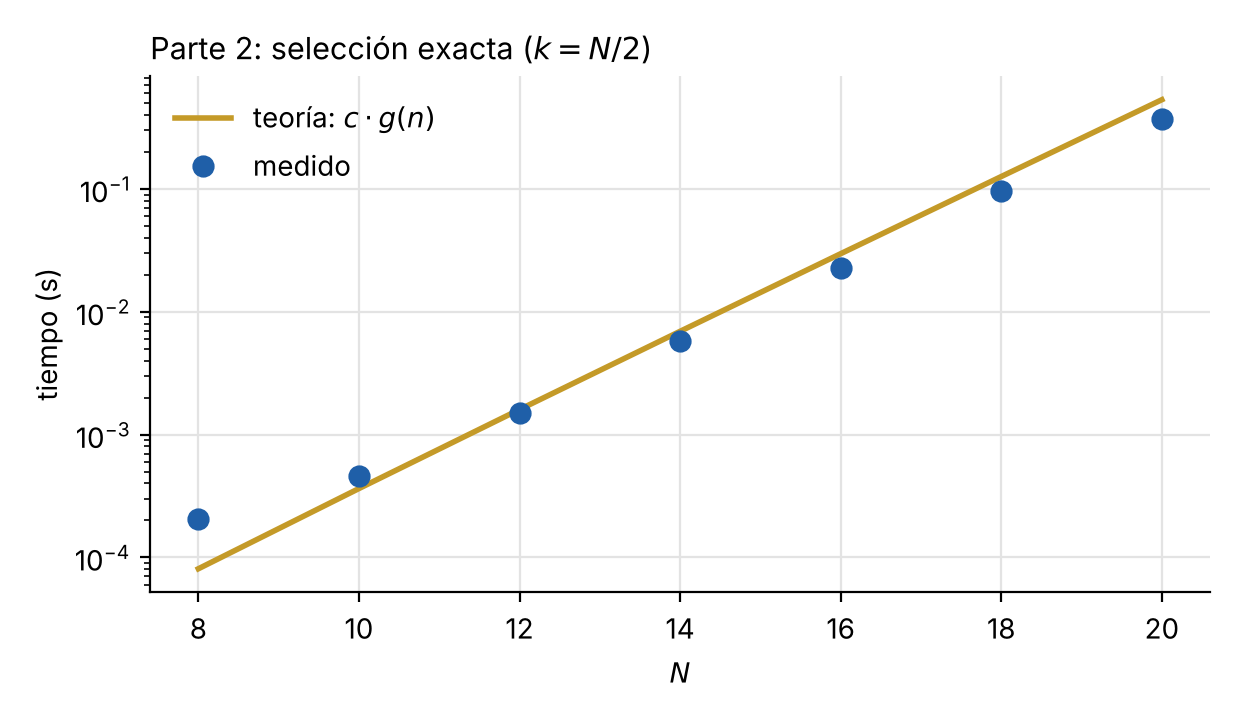
\includegraphics[width=0.6\linewidth]{img/exacto.png}
% \caption{Selección exacta: tiempo medido frente a $c\cdot\binom{N}{N/2}\frac{N}{2}$ (escala semilogarítmica).}
% \label{fig:exacto}
% \end{figure}

% \paragraph{Análisis.} El número de evaluaciones medido es \textbf{exactamente} $\binom{N}{k}$ en todos los casos, como predice la recurrencia de Pascal. En escala semilogarítmica los puntos forman casi una recta: cada vez que $N$ aumenta en 2, el tiempo se multiplica aproximadamente por 4, es decir, crece como $2^N$. Pasar de $N=8$ a $N=20$ multiplica el tiempo por más de $1800$. El cociente $r$ es mayor para $N$ pequeño, donde dominan los costos fijos de las llamadas recursivas, y se estabiliza en $\approx2.2\times10^{-7}$ a partir de $N=14$. Extrapolando, $N=40$ con $k=20$ requeriría $\binom{40}{20}\approx1.4\times10^{11}$ evaluaciones, varios días de cómputo, mientras que el voraz resuelve $N=16\,000$ en menos de medio segundo.

% %% ---------------------------------------------------------------------
% \subsection{Parte 2: verificación de la cota \texorpdfstring{$(1-1/e)$}{(1-1/e)}}

% Como pide el enunciado, la cota del Teorema~\ref{teo:nwf} se verificó calculando el óptimo por fuerza bruta. Para cada configuración $(N,k)$ se generaron 100 instancias con $|U|=25$ y $|S_j|\in[2,7]$, y se calculó la razón $f(A_g)/f(A^*)$.

% \begin{table}[H]
% \centering
% \caption{Razón entre la utilidad del voraz y la óptima (100 instancias por fila).}
% \begin{tabular}{rrrrrr}
% \toprule
% \rowcolor{uccielo} $N$ & $k$ & instancias & razón mínima & razón media & veces óptimo \\
% \midrule
% 10 & 3 & 100 & 0.875 & 0.984 & 80 \\
% 12 & 4 & 100 & 0.895 & 0.985 & 76 \\
% 14 & 5 & 100 & 0.905 & 0.986 & 71 \\
% 16 & 6 & 100 & 0.909 & 0.985 & 71 \\
% 18 & 6 & 100 & 0.913 & 0.979 & 62 \\
% \bottomrule
% \end{tabular}
% \end{table}

% \begin{figure}[H]
% \centering
% 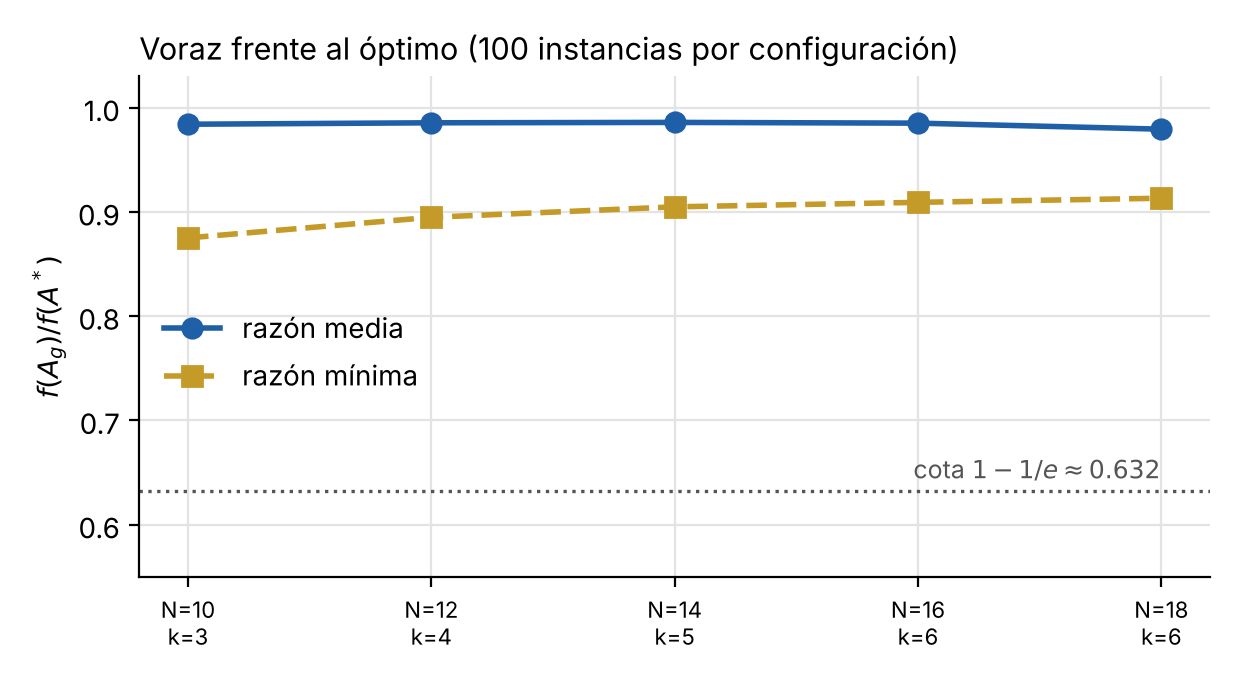
\includegraphics[width=0.65\linewidth]{img/razon.png}
% \caption{Razón media y mínima frente a la cota $1-1/e$.}
% \label{fig:razon}
% \end{figure}

% \paragraph{Análisis.} En las 500 instancias la razón fue siempre mayor que $1-1/e\approx0.632$; la peor fue $0.875$. La cota se cumple con amplio margen: es una garantía para el peor caso posible, y las instancias aleatorias están lejos de ese peor caso. El voraz no siempre es óptimo: falló entre el 20\,\% y el 38\,\% de las veces, lo cual es consistente con la NP-dureza. Un ejemplo pequeño donde falla es $S_1=\{1,2,3,4\}$, $S_2=\{1,2,5\}$, $S_3=\{3,4,6\}$ con $k=2$: el voraz elige $S_1$ primero y obtiene $5$, mientras que el óptimo $\{S_2,S_3\}$ cubre $6$ (razón $5/6$).
% }
